
After being translated, a protein undergoes several processes before becoming mature. 5 important post-translational processes can be isolated (Figure \ref{fig:pTP}), even though they may occur in parallel. 3 processes are common to cytosolic, membrane and secreted proteins, namely
\begin{itemize}
\item Deformylation and demethylation.
\item Folding.
\item Residue modifications.
\end{itemize}

Moreover, there are 2 processes that specifically target membrane and secreted proteins
\begin{itemize}
\item Translocation.
\item Cleavage of the peptide signal and lipoprotein diacylglyceryl adduction.
\end{itemize}

\begin{figure}[!ht]
\centering
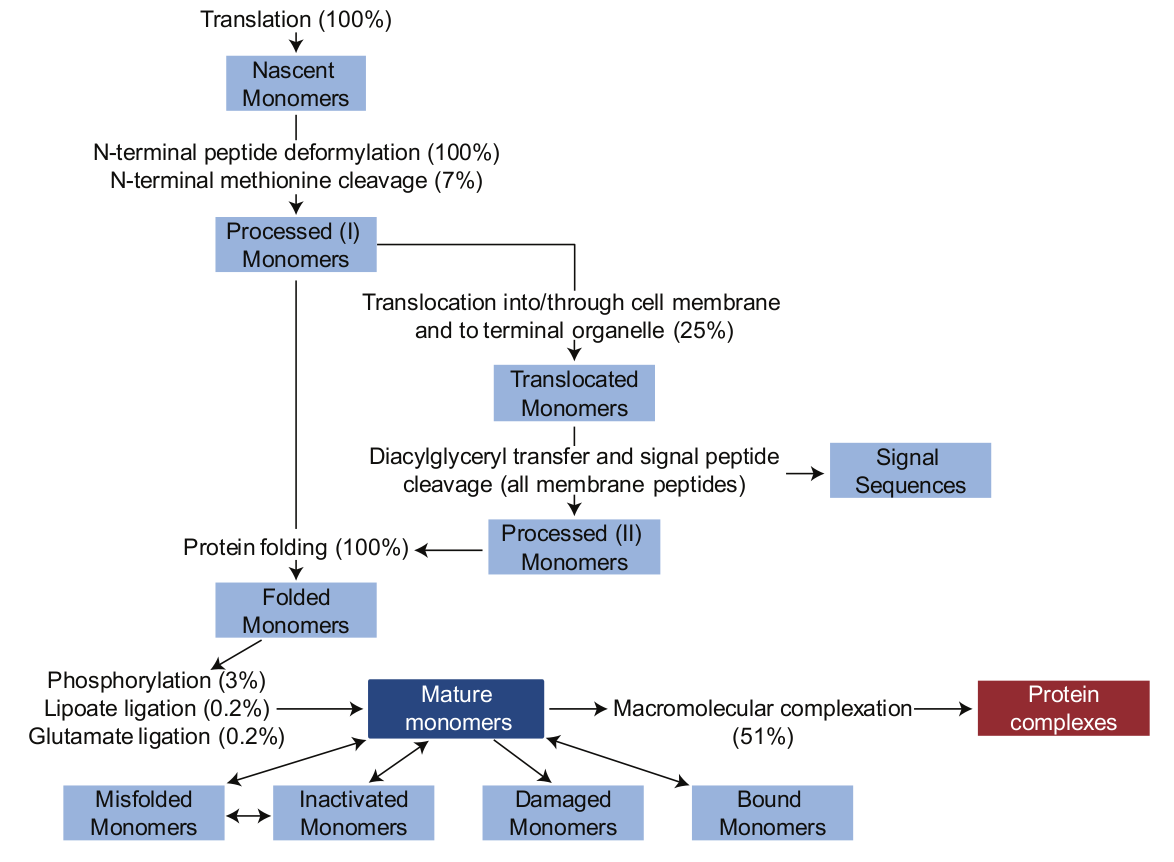
\includegraphics[width=0.8\linewidth]{figure/proteinProcesses}
\caption{Processes undergone by protein following translation (from Karr \textit{et al.})}
\label{fig:pTP}
\end{figure}

\subsubsection{Deformylation and demethylation}

For every protein, translation begins with a formylmethionine (fMet) residue. Several authors suggest that using exclusively fMet to start protein translation may be a way to regulate protein synthesis, as fMet is one of the most expensive amino acids to synthesize. Thus global protein synthesis levels would depend on global cell health.

This residue is then partially removed, but the role of deformylation and demethylation remains poorly understood. It may help in recycling fMet and influence protein degradation. According to the N-end rule, some N-terminal residues will lead to enhanced degradation. By changing the nature of the N-terminal residue, deformylation and demethylation allows for the N-end pathway to catalyze protein degradation.

Peptide deformylases (PDF) remove the formyl residue from fMet for most proteins. In \textit{B. subtilis}, YkrB is the main PDF, even though Def is known to have a similar action. It remains unclear whether these enzymes act during protein translation or after translation is completed. Methionine cleavage is performed by Methionine Aminopeptidases (MAP) but, contrarily to deformylation, it only targets a minority of proteins.

\subsubsection{Protein folding}

After translation, proteins can be viewed as a one-dimensional chain of amino acids. In order to acquire their functional form, proteins need to adopt a specific three-dimensional folding. Even though this folding is energetically favorable, numerous proteins need the help of another protein to adopt the proper conformation. These helper proteins are called chaperones. Bacteria use several chaperones. For example, in \textit{B. subtilis}
\begin{itemize}
\item The trigger factor Tig is known to assist early folding.
\item GroEL and its co-enzyme GroES assist late folding of short proteins.
\item DnaK, DnaJ and GrpE assist late folding of longer proteins.
\item FtsH may assist membrane protein folding.
\item Some proteins have specific chaperones (for example the translocated proteins TorA and NiFe are chaperoned by TorD and HybE respectively).
\end{itemize}

The trigger Factor (abbreviated Tig or TF) is an ATP-dependent protein responsible for folding assistance of nascent proteins by associating with the ribosome. It seems that it does not associate during the first steps of translation (maybe because of deformylation, demethylation or peptide signal recognition). 60 to 70\% of proteins may be in their native conformation after translation and binding by TF \citet{castanie-cornet_chaperone_2014}. Despite its large action spectrum, TF is not an essential protein as it does not seem to be responsible for folding of vital proteins and its action can be supplemented by other chaperones.

DnaK is part of the family of Heat Shock Proteins (it is a homolog of Hsp70). It is an ATP-dependent chaperone responsible for the folding of 5 to 18\% of newly synthesized proteins \citep{mayer_molecular_2000}. As part of the heat shock response it is also responsible for desaggregating and refolding proteins. This is particularly true for large proteins: 80\% of proteins >70kDa aggregate during heat shocks and even at 37°C in the absence of TF and DnaK (GroEL only folds proteins <60kDa) \citep{mayer_molecular_2000}. Roughly speaking, DnaK is composed of a hydrophobic pocket composed of $\beta$-strands, an arch of a few amino acids that facilitates substrate binding, a "lid" composed of $\alpha$-helices and an ATP-binding domain \citep{mayer_molecular_2000,mayer_hsp70_2005,castanie-cornet_chaperone_2014}. When ATP is bound to DnaK, the protein is in an "open" state with a higher dissociation constant than when it is bound to APD. Cycles where DnaK associates and dissociates from ATP could therefore lead to capture-recaptures of the substrate that may induce its folding \citep{mayer_molecular_2000}. Schematically, when DnaK is bound to ATP, it is in an acceptor state. Binding to a substrate with the help of DnaJ leads to dramatically increased hydrolysis rates and trapping of the substrate. GrpE then binds to the nucleotide binding and triggers ADP release when a new ATP binds (Fig. \ref{fig:dnaK}, top)\citep{mayer_hsp70_2005}. In heat shock conditions, the cycle is similar, except there is a competition between GrpE and ClpB, another ATP-dependent chaperone that is similar to AAA+ domains of proteases (see Protein degradation below). ClpB-DnaK is supposed to trigger desaggregation and partial refolding, while GrpE may help in completing folding if necessary (Fig. \ref{fig:dnaK}, bottom) \citep{rosenzweig_unraveling_2013}. DnaK is not an essential protein, in its absence the cell remains viable but does not grow optimally. In the absence of DnaK and TF, the cell dies except if GroEL is strongly overexpressed \citep{castanie-cornet_chaperone_2014}.

\begin{figure}[!ht]
	\centering
	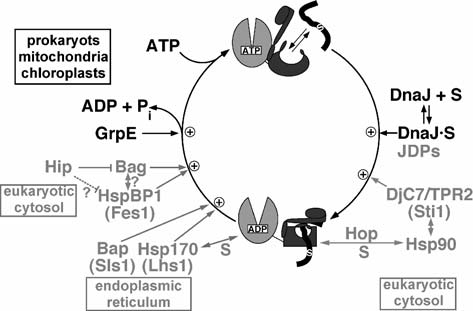
\includegraphics[width=0.4\linewidth]{figure/dnaKJE}
	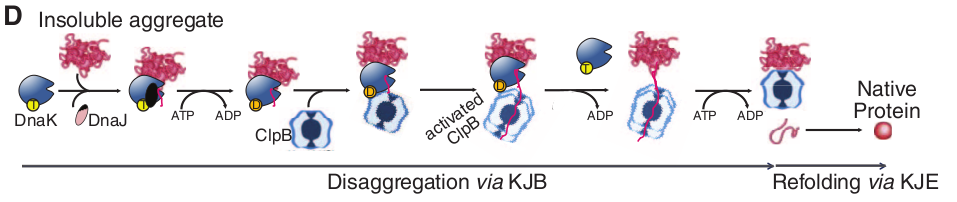
\includegraphics[width=0.8\linewidth]{figure/dnaKJB}
	\caption{One cycle of protein folding by DnaK/DnaJ/GrpE (top). Protein desaggregation and refolding by DnaK/DnaJ assisted by ClpB for desaggregation and GrpE for refolding (bottom). Figures from \citet{mayer_hsp70_2005} and \citet{rosenzweig_unraveling_2013}.}
	\label{fig:dnaK}	
\end{figure}

As DnaK, GroEL is responsible for folding and desaggregation. It folds 5 to 10\% of newly synthesized proteins  but it is only able to fold proteins whos size is in the range of 20kDa to 60 kDa \citep{castanie-cornet_chaperone_2014}. It is composed of two back-to-back heptameric cavities that can each bind 7 ATP molecules \citep{georgescauld_groel/es_2014}. When the substrate is not in excess, the cavities work in turn at a rhythm dictated by the hydrolysis of the 7 ATP molecules (Fig. \ref{fig:groESL}). The two cavities may influence each other. According to  \citet{lin_repetitive_2013}, one of the cavities is always occupied, binding of substrate to the entrance of the empty cavity releases ADP from that cavity, which enables ATP hydrolysis in the other cavity. Once ATP is hydrolysed in the occupied cavity, ATP may bind to the empty cavity and starts drawing the substrate inside and drives closing of the cavity by GroES and release of substrate in the other cavity. Folding could be linked to both substrate elongation and compaction when it enters the cavity \citep{lim_evidence_2014} or strongly charged surfaces within the cavity \citep{georgescauld_groel/es_2014}. More precisely, \citet{lim_evidence_2014} show that GroEL captures/recaptures one of its substrate at a rate that depends on the temperature (higher temperature leads to stronger ATP consumption and quicker cycling). The higher the temperature, the quicker the folding. At more than 30°C, the folding occurs quicker than pure sequestration in a mutated GroEL that does not release the substrate (and does not consume ATP), indicating a potential functional role to the capture mechanism. On the contrary, \citet{georgescauld_groel/es_2014} suggest that sequestration may be enough for a substrate that contains a TIM barrel composed of $\alpha$-helices. By positioning some of the helices through interactions with the cavity, the folding is increased 50-fold and becomes quicker than the synthesis of the protein. Through sequestration, GroEL also participates to removing protein aggregates. Although it is more specific than DnaK and TF, GroEL is an essential protein, probably because it folds essential proteins that can not be folded properly by other chaperones.

\begin{figure}[!ht]
	\centering
	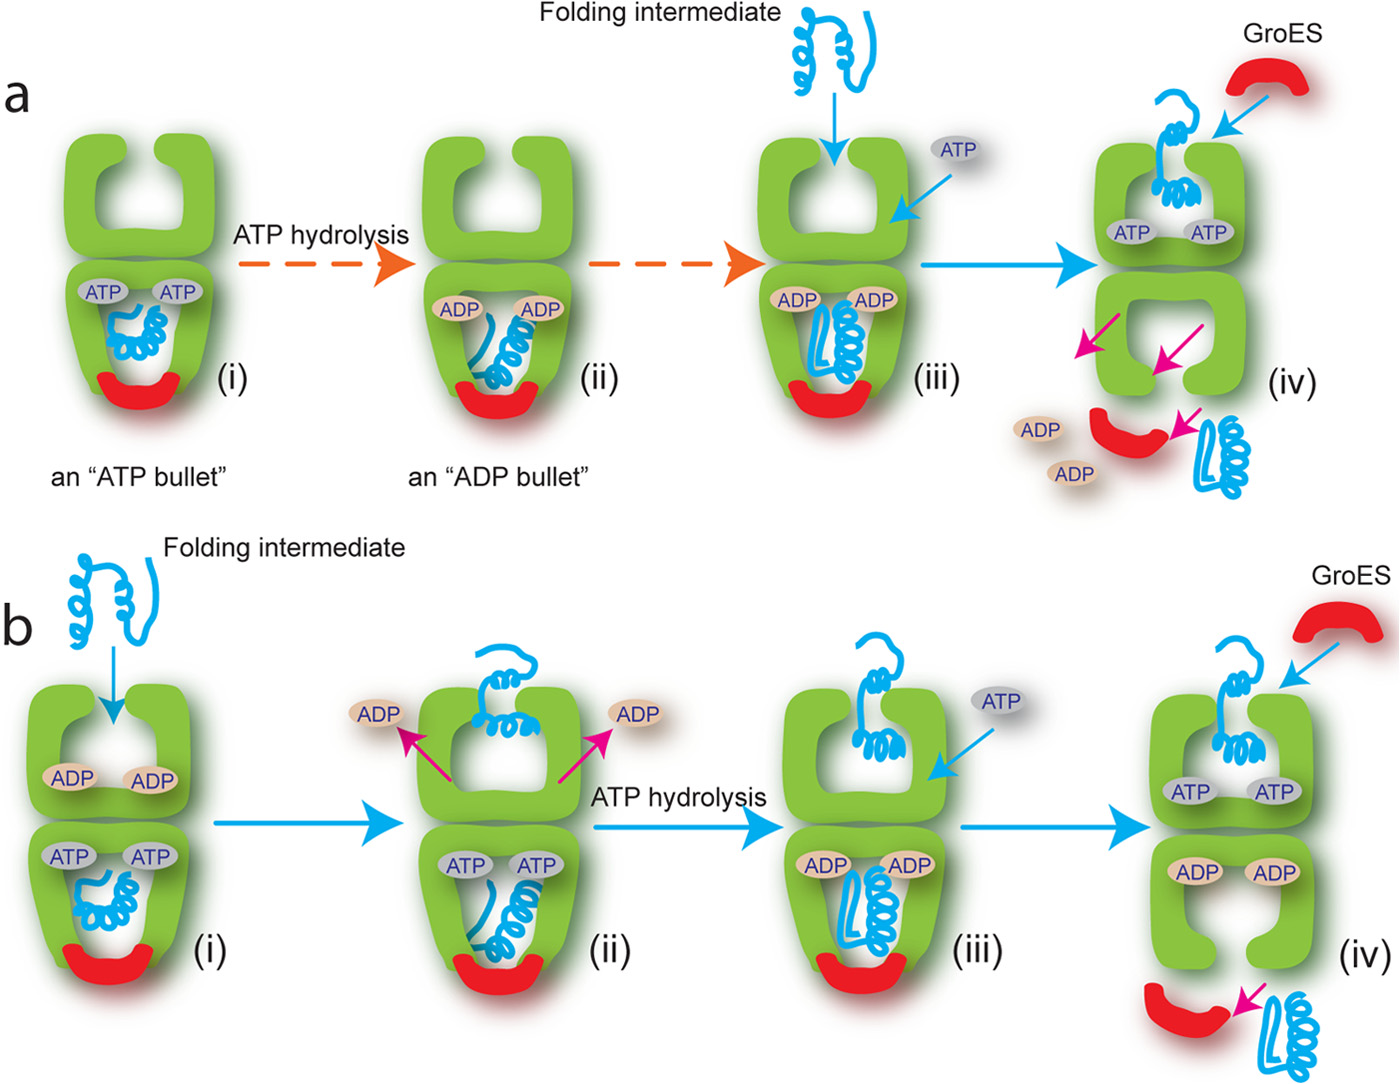
\includegraphics[width=0.8\linewidth]{figure/groESL}
	\caption{Models for cycles of protein folding by GroEL and GroES. Figure from \citet{lin_repetitive_2013}.}
	\label{fig:groESL}	
\end{figure}


\subsubsection{Translocation, peptide signal cleavage and diacylglyceryl adduction}

During its life cycle, a bacterium heavily interacts with the extracellular medium. These interactions are enabled by proteins that are embedded in the membrane (nutrient transporters, ATP synthase, receptors, transducers) or secreted (virulence factors, cell wall components). Proteins that need to undergo translocation are identified by their N-terminal and C-terminal signal sequences (petide signals). Their embedding and secretion through the hydrophobic membrane is assisted by a specific machinery. 

Two important pathways are involved in protein translocation: Tat and SecA. They both involve a docking and a translocation step. Docking is mediated by peptide signals that can be recognized by signal recognition proteins (SRP) or directly by membrane proteins involved in the translocons (such as SecA or TatC). Translocation then occurs through a pore of variable size consisting of several proteins (SecYEG translocase or TatA like proteins). Depending on the nature of the proteins, translocation can occur simultaneously to translation (integral membrane proteins) or after translation (lipoproteins and secreted proteins). 

Following translocation, lipoproteins are anchored to the membrane through ligation of diacylglyceryl mediated by diacylglyceryl transferase and their peptide signal is removed by a signal peptidase. (what about the cleavage of peptide signals of secreted proteins and integral membrane proteins in \textit{B. subtilis} ???)


\subsubsection{Residue modifications}

Some proteins undergo post-translational chemical modifications. These modifications may serve different objectives such as favoring alternative conformations or regulating protein activity. Examples of residue modifications include phosphorylation, lipoyl transfer to lysine and $\alpha$-glutamate ligation, all catalyzed by specific enzymes.

\subsubsection{Protein degradation}

Protein degradation is assured by proteases in a process called proteolysis. Proteolysis has several roles within the cell \citep{gur_regulated_2011,konovalova_regulated_2014}:
\begin{itemize}
	\item Proteolysis may degrade destructured proteins to avoid toxicity and enable amino acid recycling. However, \citet{gur_regulated_2011} argue that refolding may be the usual recycling mechanisms, as a typical \textit{E. coli} cell contains roughly 1600 and 10000 copies of chaperones GroEL and DnaK, respectively, against 50-150 copies of proteases ClpXP, ClpAP and Lon. Molecular competition for denatured substrates would therefore largely favor chaperones.
	\item Proteolysis may be used to downregulate specific protein pools. Gene and mRNA regulation does not directly impact these pools, targeted degradation allows rapid decrease of protein concentration.
	\item Proteolysis may only affect a small part of the protein. Typical examples are found in transduction, where a protein is cut in two at the level of the membrane, yielding a cytosolic part that may activate gene transcription.
\end{itemize}

There is a family of well-characterized proteases that are called AAA+ proteases (ATPases Associated with diverse cellular Activities) which are thought to act on a very large spectrum of proteins. The members are schematically composed of two parts: an AAA+ module (often a ring-shaped hexamer) that is able to unfold and translocate proteins, and a protease module (a cavity-shaped oligomer), that cuts the protein into small pieces, in an ATP independent manner (Fig. \ref{fig:proteaseStructure}) \citep{sauer_aaa+_2011}. Folded proteins cannot enter the protease chamber, the association with the AAA+ module is essential for proteolysis. This association enables targeted substrate recognition.

\begin{figure}[!ht]
	\centering
	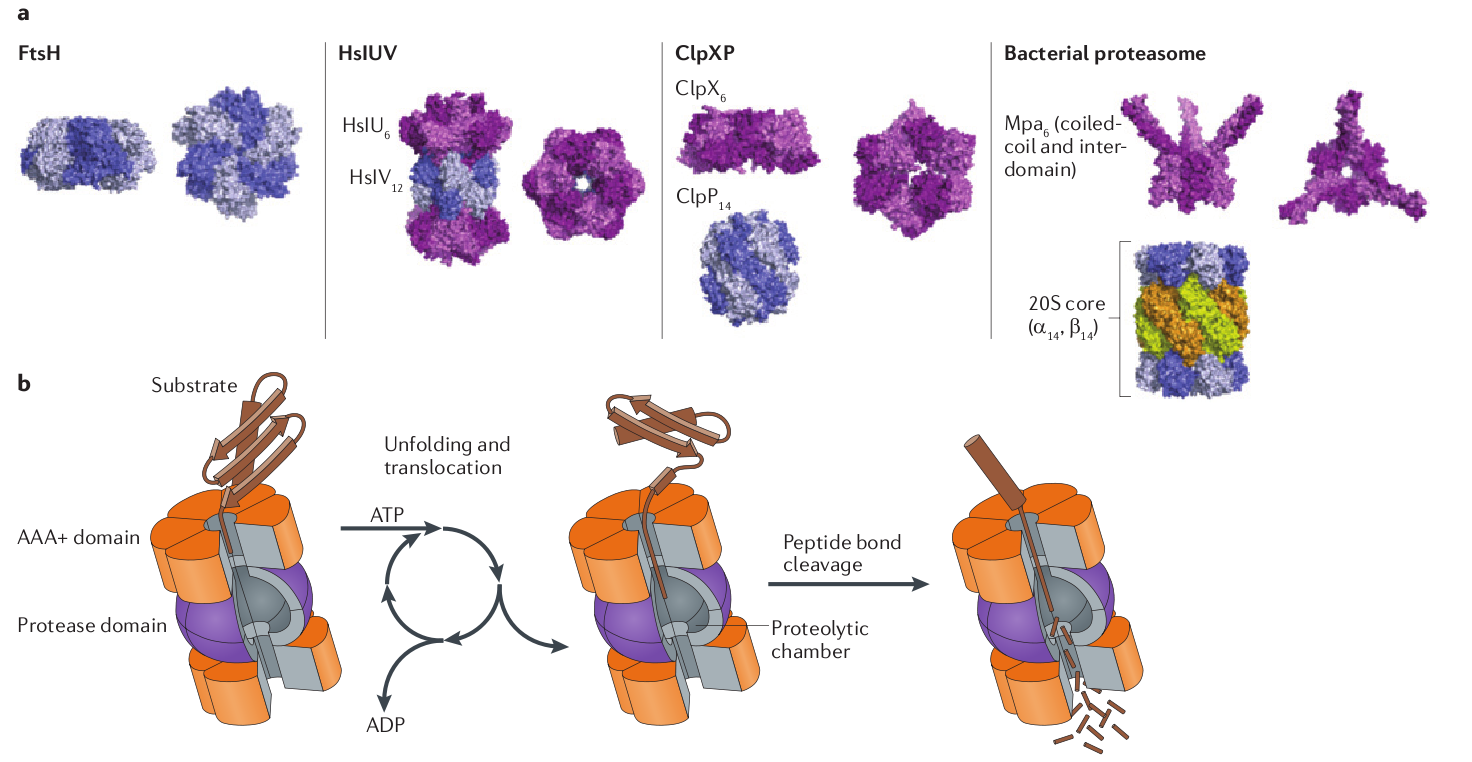
\includegraphics[width=0.8\linewidth]{figure/proteaseStructure}
	\caption{Structure of AAA+ proteases. Top: AAA+ hexamers are shown in purple, proteolytic cavities in other colors. Bottom: schematic representation of protein degradation by an assembled protease. Figure from \citet{gur_regulated_2011}.}
	\label{fig:proteaseStructure}	
\end{figure}

Figure \ref{fig:proteaseFamily} gives an overview of the main AAA+ proteases found in bacteria. The AAA+ module can be on the same protein as the protease (FtsH, Lon) or translated independently (HslU+HslV, ClpX+ClpP, ClpA/C+ClpP, PAN+20S). In the latter case, it can have a translocation activity that is independent of proteolysis, as has been shown for ClpX, or ClpA homolog ClpB (which does not associate with a protease) \citep{sauer_aaa+_2011}. The cost of translocation is difficult to evaluate. \citet{sauer_aaa+_2011} remind that, depending on the conformation, the translocation of the Tit protein can cost from 100 ATPs to 600 ATP. On ClpX 6 ATP can theoretically bind, even though it seems that only 4 can bind at the same time (because of conformation changes, 2 sites cannot be accessed) and a typical cycle alternates between 4 ATP and 3 ATP + ADP. The authors also distinguish three translocation states that influence ATP consumption: (i) protein spontaneously unfolds with traction, translocation is cooperative, (ii) protein resists to traction, leading to translocation "slippage" and wasted ATP, (iii) protein resists to traction and dissociates from the translocase. The latter case might sound dramatic at first, but it may be a functional way to distinguish between native and destructured proteins, native proteins having a much higher probability of unbinding, so only unfolded proteins are efficiently degraded.

\begin{figure}[!ht]
	\centering
	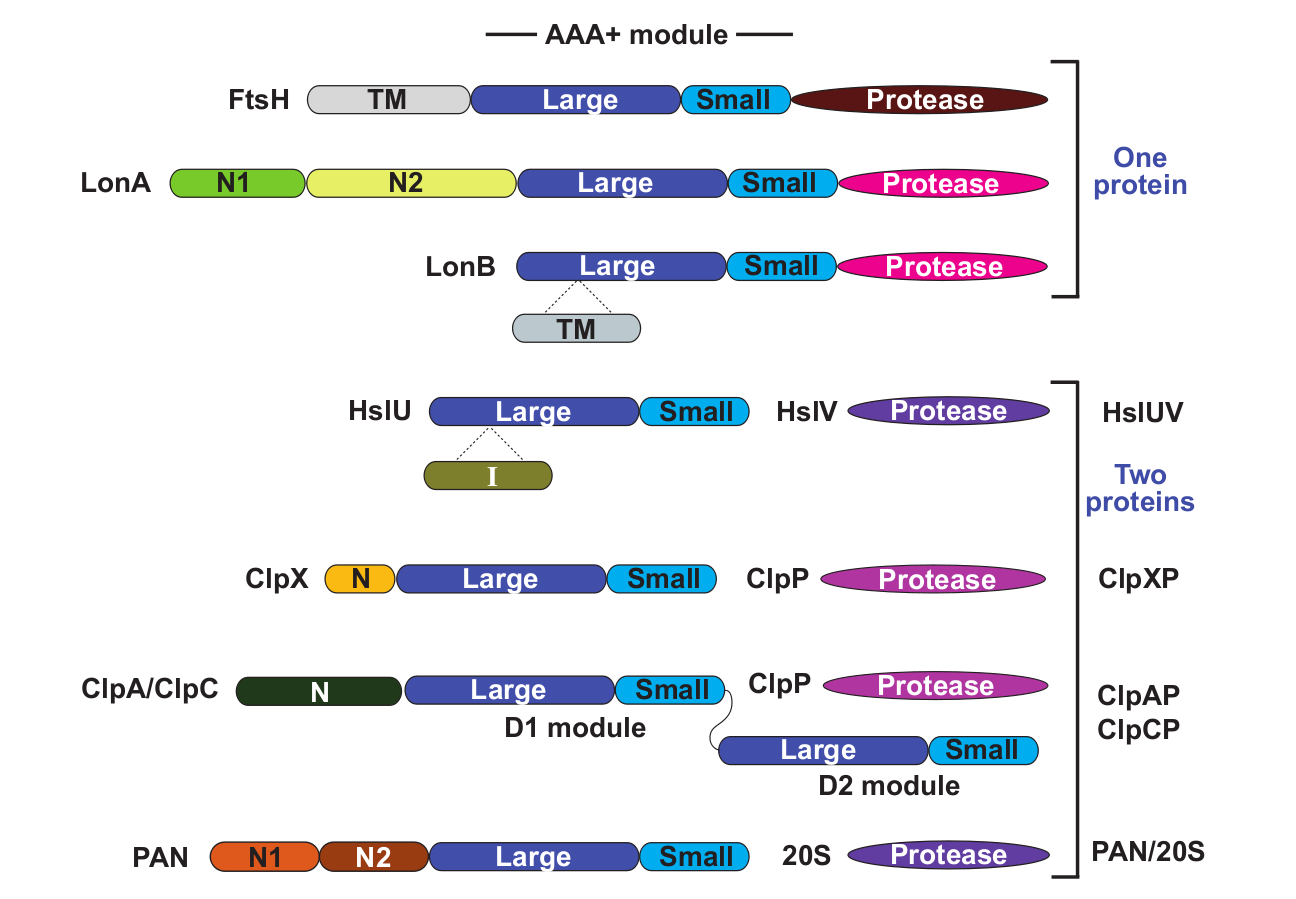
\includegraphics[width=0.8\linewidth]{figure/proteaseFamily}
	\caption{Phylogeny of the main AAA+ proteases. Top bracket: proteases where the AAA+ module and the proteolytic cavity are within a single protein. Bottom bracket: proteases where AAA+ module(s) and proteolytic cavity are separated. Colors indicate homologous domains (AAA+ modules are particularly well conserved). Figure from \citet{sauer_aaa+_2011}.}
	\label{fig:proteaseFamily}	
\end{figure}

A protein may be degraded only if it is recognized by the AAA+ module. The recognition is mediated by a degradation tag (often referred to as degron). \citet{sauer_aaa+_2011} distinguish four essential mechanisms in substrate recognition:
\begin{itemize}
	\item \textbf{Cryptic degron}: a sequence of amino acids within the protein that is accessible only in specific conditions, e.g. the protein is unfolded.
	\item \textbf{Amino acid appendage}: a sequence of amino acids that is recognized by a protease is added to the protein. A typical example is the SsrA tag: when a ribosome stalls, a tmRNA is loaded and the ribosome translates the tmRNA instead of the original mRNA. The amino acid sequence coded by the tmRNA is termed SsrA tag and is specifically recognized by ClpXP.
	\item \textbf{N-end rule}: the mechanism here is not totally understood, but the presence of some amino acids at the N-terminal end influence degradation, namely leucine (L), phenylalanine (F), tryptophane (W) and tyrosine (Y) \citep{sauer_aaa+_2011,tasaki_n-end_2012}. This process is mediated by ClpS and allows recognition by ClpAP, even though the details are unclear \citep{roman-hernandez_clps_2011,sauer_aaa+_2011,tasaki_n-end_2012}. Protein could be tagged for degradation by cleaving the initial methionine or by changing the N-terminal residue by specific enzymes (which target specific amino acids, called secondary targets, see Fig.~\ref{fig:nEndRule}).
	\item \textbf{Adaptator proteins}: these proteins serves as intermediates between the substrate and the protease, e.g. ClpS connects N-end rule degrons to ClpAP, SspB connects SsrA degrons to ClpXP. This allows for numerous regulation possibilities (competition between adaptators for a protease, antiadaptators).
\end{itemize}

\begin{figure}[!ht]
	\centering
	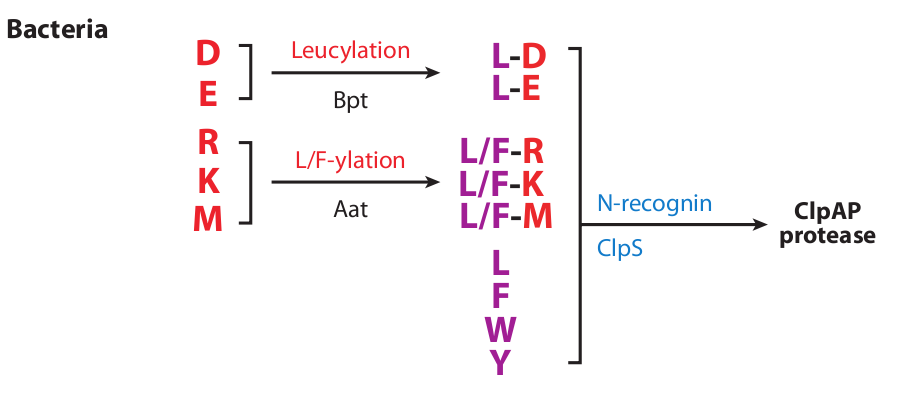
\includegraphics[width=0.4\linewidth]{figure/nEndRule}
	\caption{Primary targets (purple) and secondary targets (red) of the N-end rule pathway. The main proteins responsible for each process is indicated next to each arrow. Figure from \citet{tasaki_n-end_2012}.}
	\label{fig:nEndRule}	
\end{figure}

